\clearpage

\section{Detailed comparison of VaLOR and Prob3++ oscillation probabilities}
\label{appendix:comparison_with_prob3}

%
% numu->numu
%

\begin{figure}[ht]
\begin{minipage}[t]{0.48\linewidth}
\centering
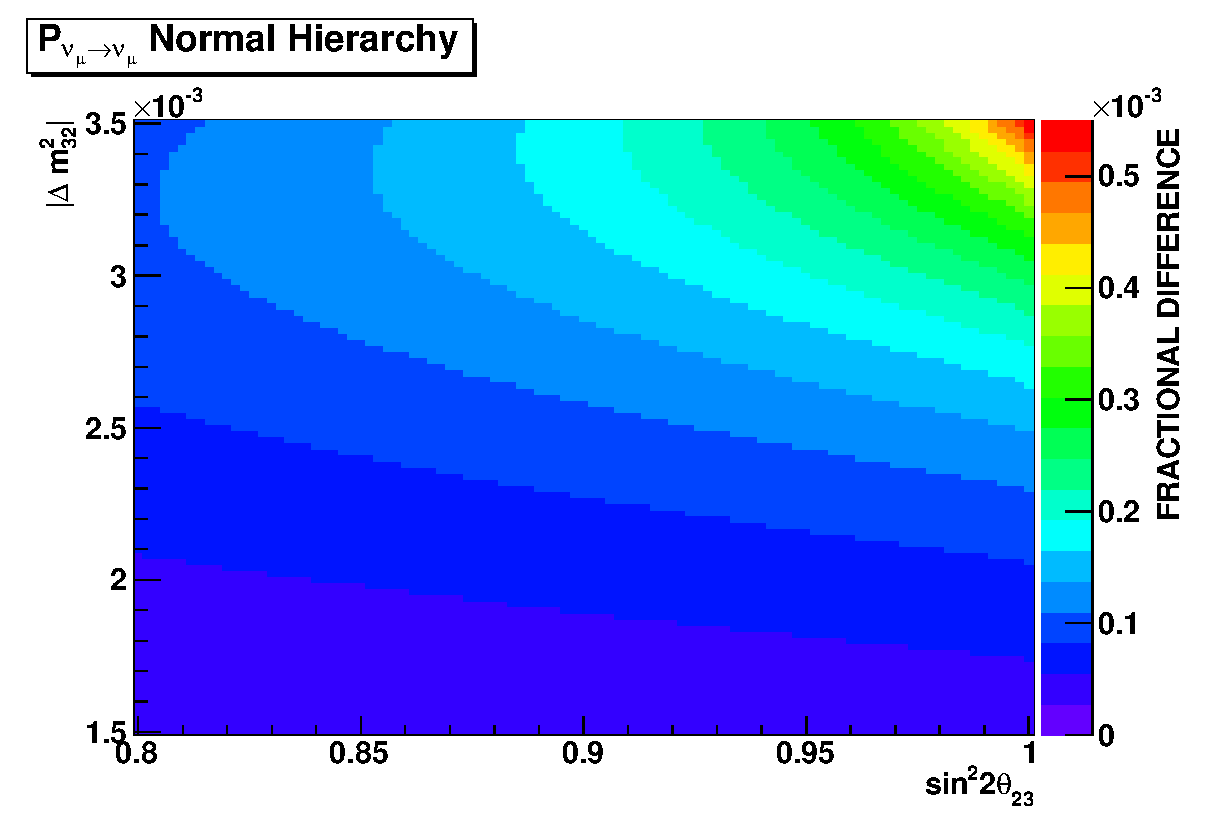
\includegraphics[width=18pc,height=18pc]{./images/osc_prob/prob3_comparison/ComparisonNuMuToNuMuNH.eps}
\caption{
  Comparison of the VaLOR $\nu_{\mu}\rightarrow\nu_{\mu}$ oscillation probabilities in matter with those obtained from Prob3++ 
  as a function of $\sin^{2}2\theta_{23}$ and $|\Delta m_{32}^{2}|$ for E$_{\nu}$ = 1 GeV; normal mass hierarchy, 
  $\sin^{2}2\theta_{13}$ = 0.1, $\sin^{2}2\theta_{12}$ = 0.8704, $\Delta m_{21}^{2}$ = 7.6$\times$10$^{-5}$ eV$^{2}$/c$^{4}$,
  $\delta_{CP}$ = 0 and Earth crust density = 2.6 g/cm$^{3}$.
}
\label{fig:comp_valor_prob3pp_nh_numu_numu}
\end{minipage}
\hspace{0.06\linewidth}
\begin{minipage}[t]{0.48\linewidth}
\centering  
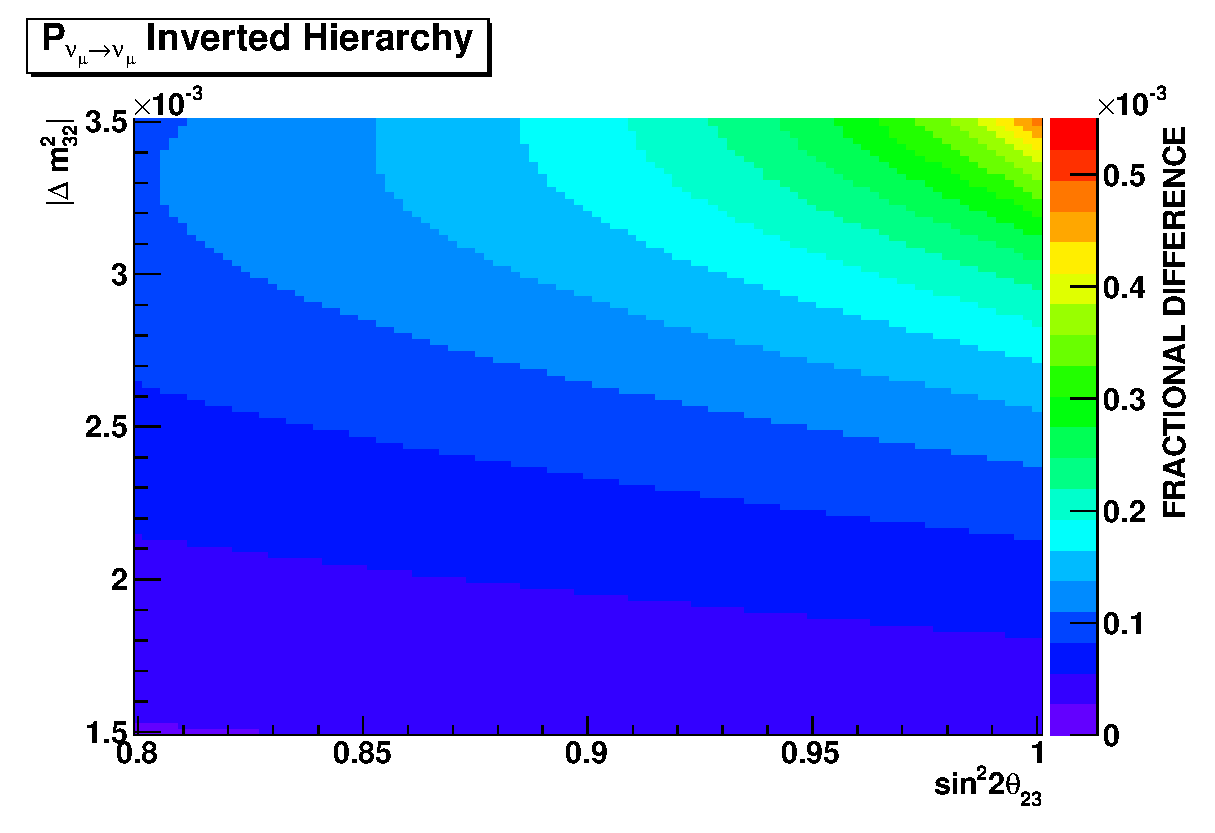
\includegraphics[width=18pc,height=18pc]{./images/osc_prob/prob3_comparison/ComparisonNuMuToNuMuIH.eps}
\caption{
  Comparison of the VaLOR $\nu_{\mu}\rightarrow\nu_{\mu}$ oscillation probabilities in matter with those obtained from Prob3++ 
  as a function of $\sin^{2}2\theta_{23}$ and $|\Delta m_{32}^{2}|$ for E$_{\nu}$ = 1 GeV; inverted mass hierarchy, 
  $\sin^{2}2\theta_{13}$ = 0.1, $\sin^{2}2\theta_{12}$ = 0.8704, $\Delta m_{21}^{2}$ = 7.6$\times$10$^{-5}$ eV$^{2}$/c$^{4}$,
  $\delta_{CP}$ = 0 and Earth crust density = 2.6 g/cm$^{3}$.
}
\label{fig:comp_valor_prob3pp_nh_numu_numu}
\end{minipage}
\end{figure}


%
% numubar -> numubar
%

\begin{figure}[ht]
\begin{minipage}[t]{0.47\linewidth}
\centering
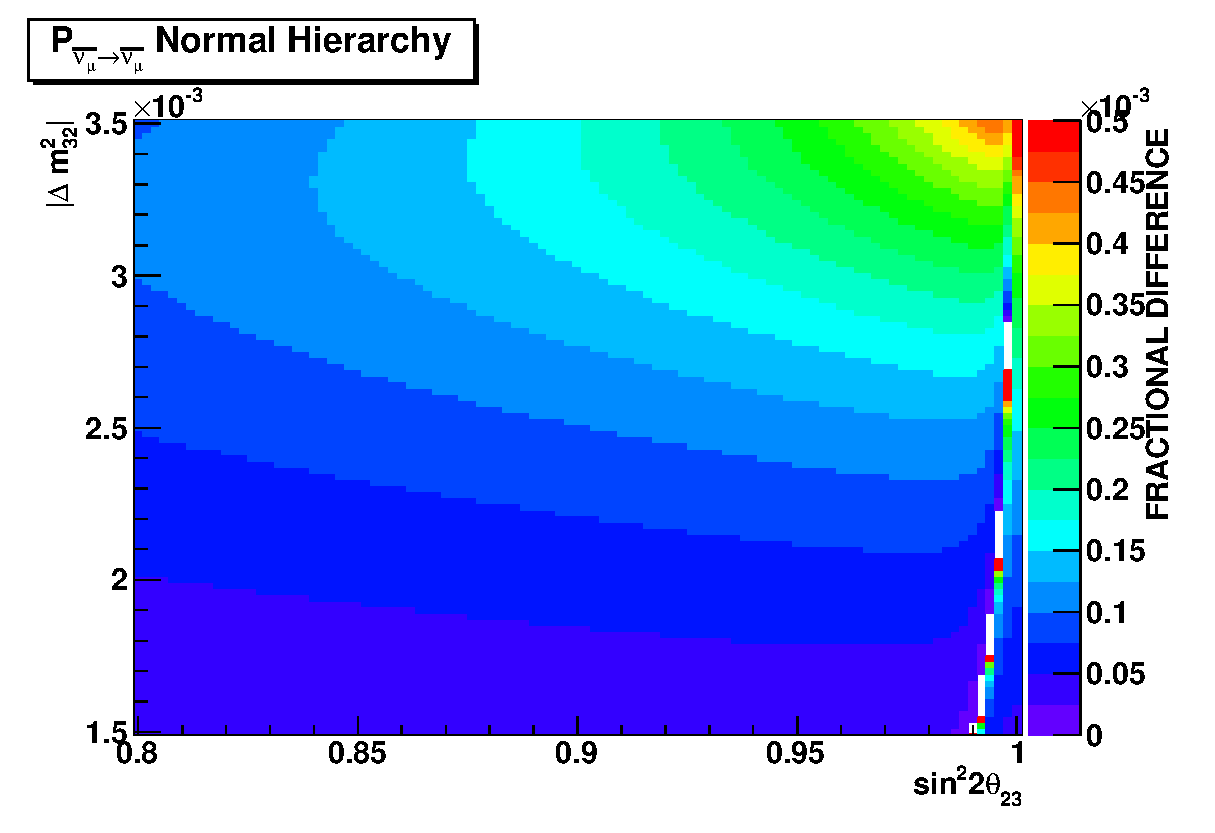
\includegraphics[width=18pc,height=18pc]{./images/osc_prob/prob3_comparison/ComparisonNuMuBarToNuMuBarNH.eps}
\caption{
  Comparison of the VaLOR $\bar{\nu}_{\mu}\rightarrow\bar{\nu}_{\mu}$ oscillation probabilities in matter with those obtained from Prob3++ 
  as a function of $\sin^{2}2\theta_{23}$ and $|\Delta m_{32}^{2}|$ for E$_{\nu}$ = 1 GeV; normal mass hierarchy, 
  $\sin^{2}2\theta_{13}$ = 0.1, $\sin^{2}2\theta_{12}$ = 0.8704, $\Delta m_{21}^{2}$ = 7.6$\times$10$^{-5}$ eV$^{2}$/c$^{4}$,
  $\delta_{CP}$ = 0 and Earth crust density = 2.6 g/cm$^{3}$.
}
\label{fig:comp_valor_prob3pp_nh_numubar_numubar}
\end{minipage}
\hspace{0.06\linewidth}
\begin{minipage}[t]{0.47\linewidth}
\centering  
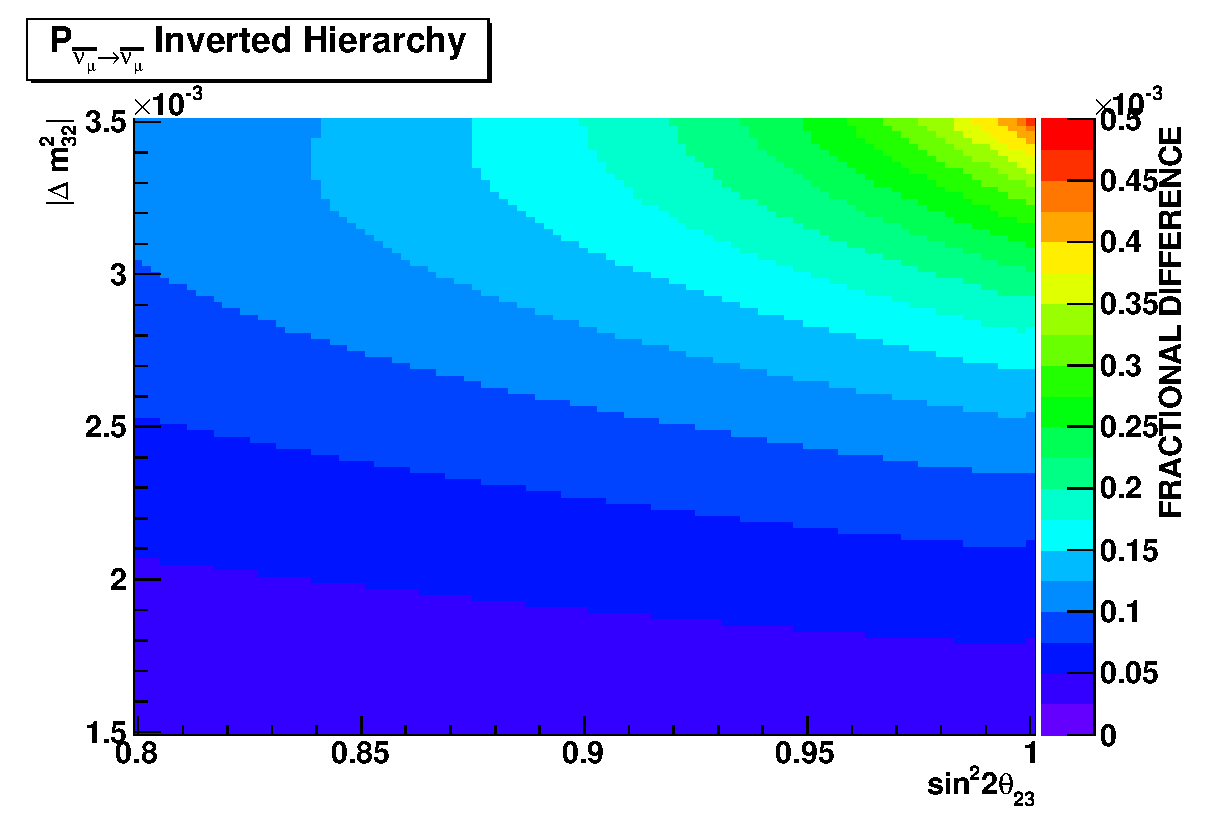
\includegraphics[width=18pc,height=18pc]{./images/osc_prob/prob3_comparison/ComparisonNuMuBarToNuMuBarIH.eps}
\caption{
  Comparison of the VaLOR $\bar{\nu}_{\mu}\rightarrow\bar{\nu}_{\mu}$ oscillation probabilities in matter with those obtained from Prob3++ 
  as a function of $\sin^{2}2\theta_{23}$ and $|\Delta m_{32}^{2}|$ for E$_{\nu}$ = 1 GeV; inverted mass hierarchy, 
  $\sin^{2}2\theta_{13}$ = 0.1, $\sin^{2}2\theta_{12}$ = 0.8704, $\Delta m_{21}^{2}$ = 7.6$\times$10$^{-5}$ eV$^{2}$/c$^{4}$,
  $\delta_{CP}$ = 0 and Earth crust density = 2.6 g/cm$^{3}$.
}
\label{fig:comp_valor_prob3pp_nh_numubar_numubar}
\end{minipage}
\end{figure}


%
% nue -> nue
%

\begin{figure}[ht]
\begin{minipage}[t]{0.47\linewidth}
\centering
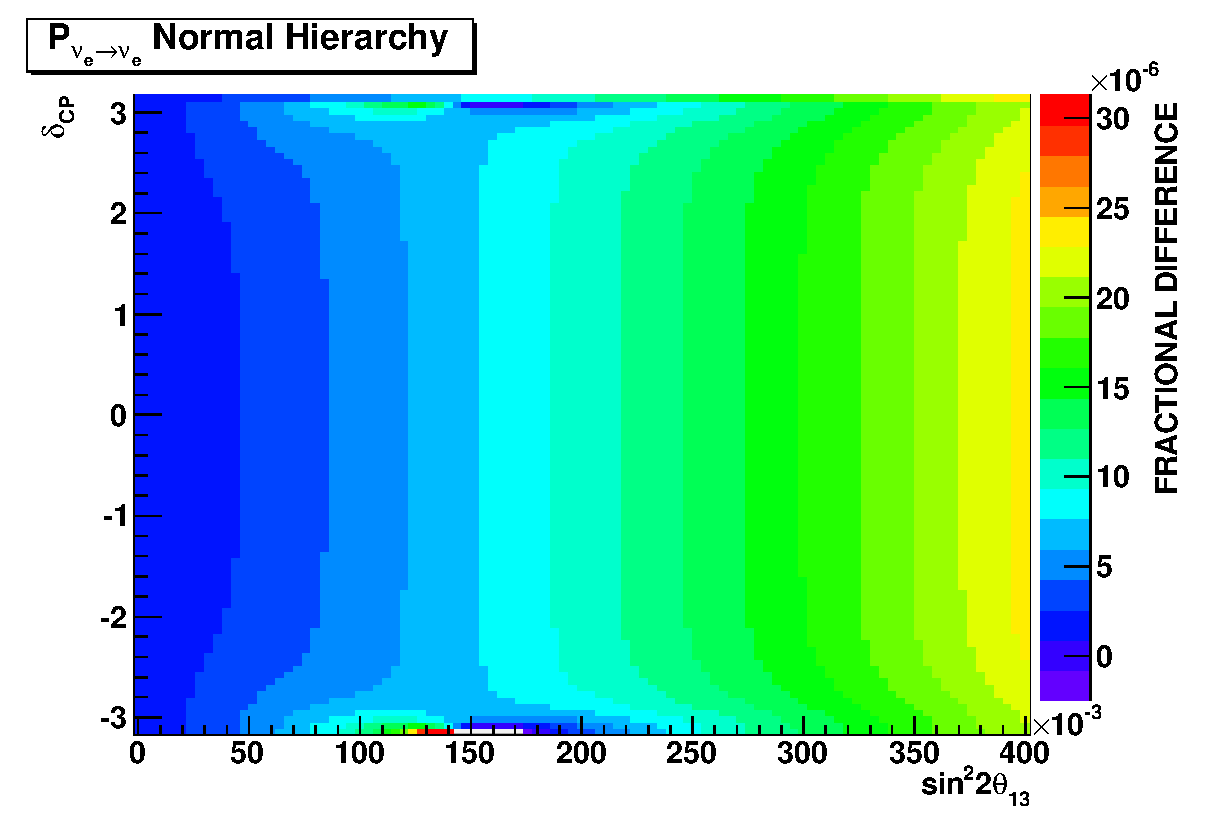
\includegraphics[width=18pc,height=18pc]{./images/osc_prob/prob3_comparison/ComparisonNuEToNuENH.eps}
\caption{
  Comparison of the VaLOR $\nu_{e}\rightarrow\nu_{e}$ oscillation probabilities in matter with those obtained from Prob3++ 
  as a function of $\sin^{2}2\theta_{13}$ and $\delta_{CP}$ for E$_{\nu}$ = 1 GeV; normal mass hierarchy, 
  $\sin^{2}2\theta_{23}$ = 1.0, $|\Delta m_{32}^{2}|$ = 2.4$\times$10$^{-3}$ eV$^{2}$/c$^{4}$, $\sin^{2}2\theta_{12}$ = 0.8704,
  $\Delta m_{21}^{2}$ = 7.6$\times$10$^{-5}$ eV$^{2}$/c$^{4}$ and Earth crust density = 2.6 g/cm$^{3}$.
}
\label{fig:comp_valor_prob3pp_nh_nue_nue}
\end{minipage}
\hspace{0.06\linewidth}
\begin{minipage}[t]{0.47\linewidth}
\centering  
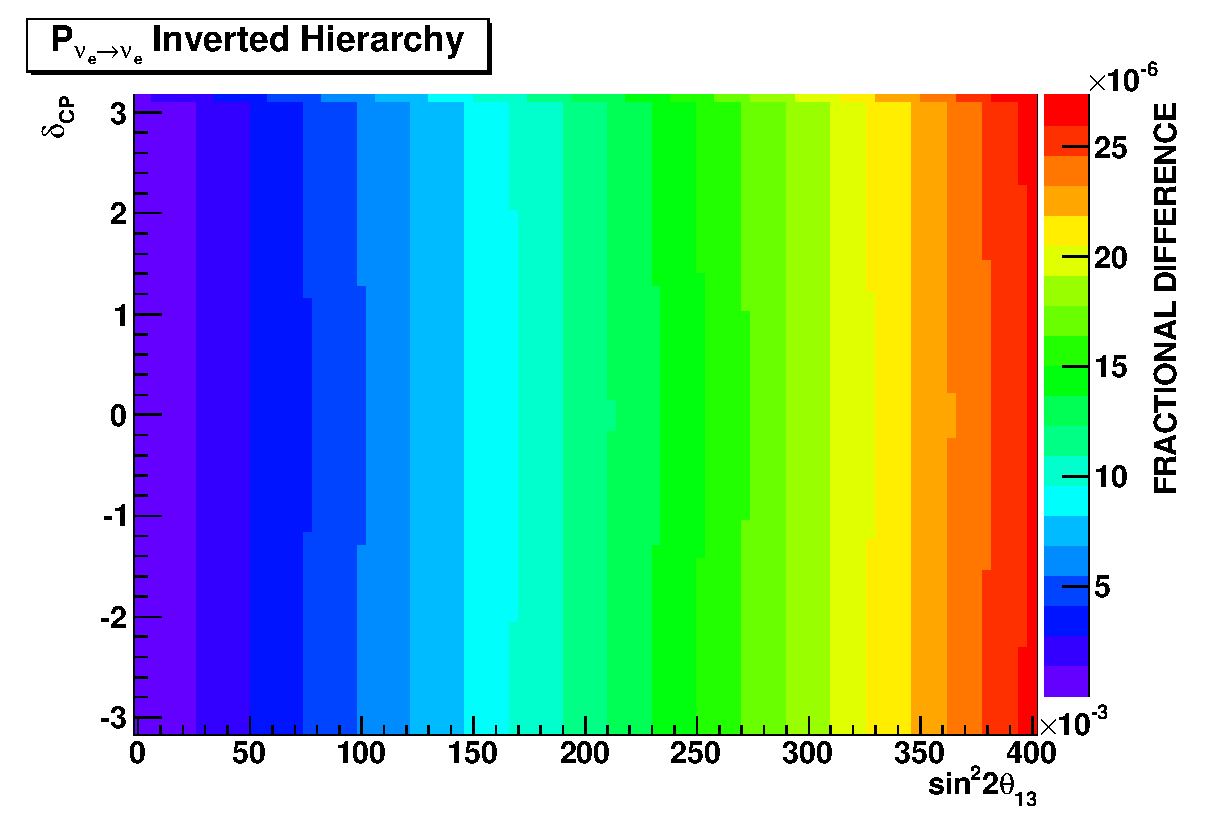
\includegraphics[width=18pc,height=18pc]{./images/osc_prob/prob3_comparison/ComparisonNuEToNuEIH.eps}
\caption{
  Comparison of the VaLOR $\nu_{e}\rightarrow\nu_{e}$ oscillation probabilities in matter with those obtained from Prob3++ 
  as a function of $\sin^{2}2\theta_{13}$ and $\delta_{CP}$ for E$_{\nu}$ = 1 GeV; inverted mass hierarchy, 
  $\sin^{2}2\theta_{23}$ = 1.0, $|\Delta m_{32}^{2}|$ = 2.4$\times$10$^{-3}$ eV$^{2}$/c$^{4}$, $\sin^{2}2\theta_{12}$ = 0.8704,
  $\Delta m_{21}^{2}$ = 7.6$\times$10$^{-5}$ eV$^{2}$/c$^{4}$ and Earth crust density = 2.6 g/cm$^{3}$.
}
\label{fig:comp_valor_prob3pp_nh_nue_nue}
\end{minipage}
\end{figure}


%
% nuebar -> nuebar
%

\begin{figure}[ht]
\begin{minipage}[t]{0.47\linewidth}
\centering
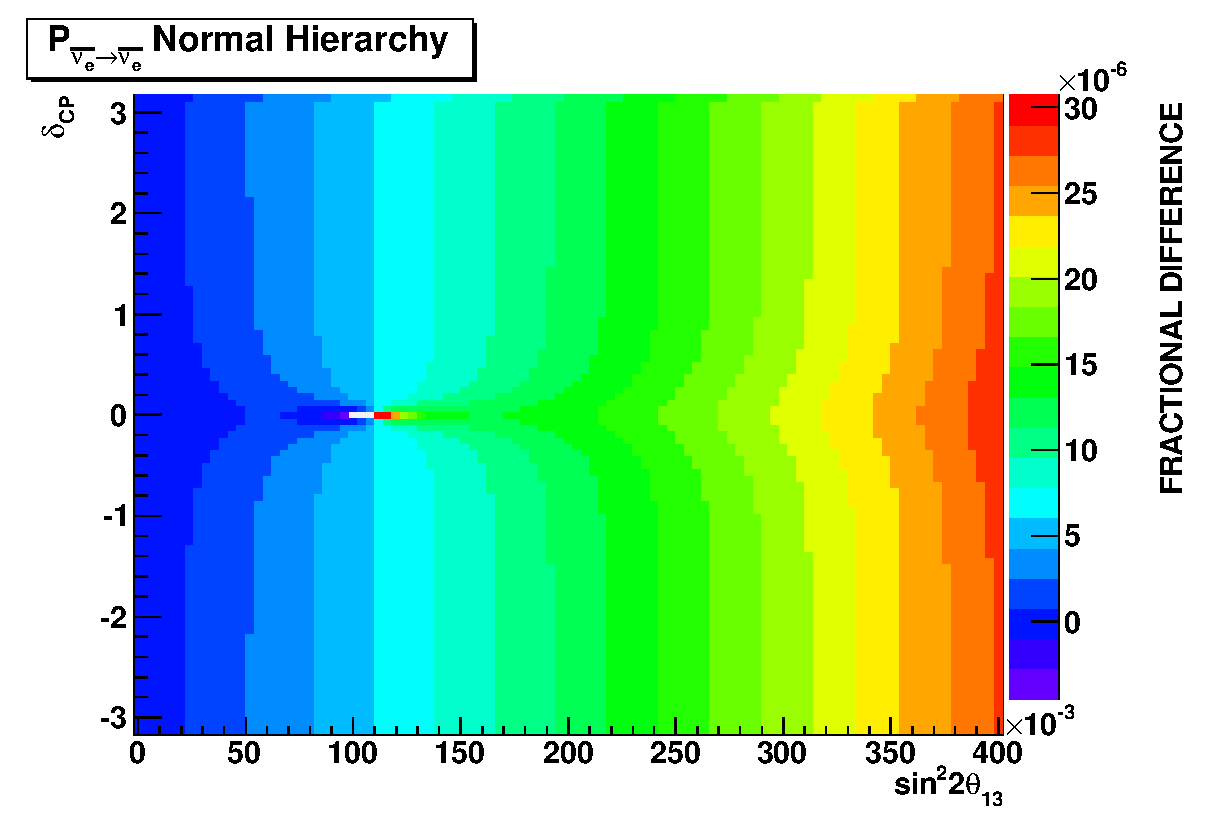
\includegraphics[width=18pc,height=18pc]{./images/osc_prob/prob3_comparison/ComparisonNuEBarToNuEBarNH.eps}
\caption{
  Comparison of the VaLOR $\bar{\nu}_{e}\rightarrow\bar{\nu}_{e}$ oscillation probabilities in matter with those obtained from Prob3++ 
  as a function of $\sin^{2}2\theta_{13}$ and $\delta_{CP}$ for E$_{\nu}$ = 1 GeV; normal mass hierarchy, 
  $\sin^{2}2\theta_{23}$ = 1.0, $|\Delta m_{32}^{2}|$ = 2.4$\times$10$^{-3}$ eV$^{2}$/c$^{4}$, $\sin^{2}2\theta_{12}$ = 0.8704,
  $\Delta m_{21}^{2}$ = 7.6$\times$10$^{-5}$ eV$^{2}$/c$^{4}$ and Earth crust density = 2.6 g/cm$^{3}$.
}
\label{fig:comp_valor_prob3pp_nh_nuebar_nuebar}
\end{minipage}
\hspace{0.06\linewidth}
\begin{minipage}[t]{0.47\linewidth}
\centering  
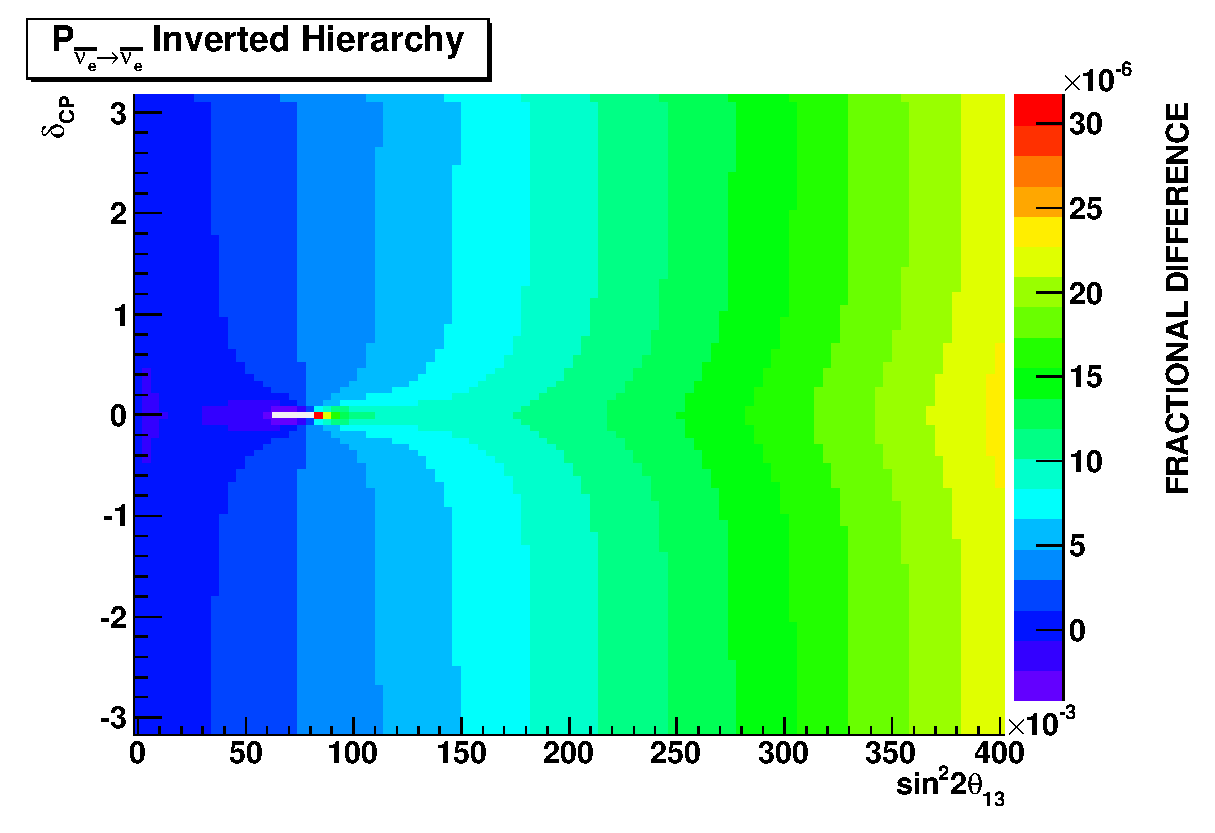
\includegraphics[width=18pc,height=18pc]{./images/osc_prob/prob3_comparison/ComparisonNuEBarToNuEBarIH.eps}
\caption{
  Comparison of the VaLOR $\bar{\nu}_{e}\rightarrow\bar{\nu}_{e}$ oscillation probabilities in matter with those obtained from Prob3++ 
  as a function of $\sin^{2}2\theta_{13}$ and $\delta_{CP}$ for E$_{\nu}$ = 1 GeV; inverted mass hierarchy, 
  $\sin^{2}2\theta_{23}$ = 1.0, $|\Delta m_{32}^{2}|$ = 2.4$\times$10$^{-3}$ eV$^{2}$/c$^{4}$, $\sin^{2}2\theta_{12}$ = 0.8704,
  $\Delta m_{21}^{2}$ = 7.6$\times$10$^{-5}$ eV$^{2}$/c$^{4}$ and Earth crust density = 2.6 g/cm$^{3}$.
}
\label{fig:comp_valor_prob3pp_nh_nuebar_nuebar}
\end{minipage}
\end{figure}

%
% numu -> nue
%

\begin{figure}[ht]
\begin{minipage}[t]{0.47\linewidth}
\centering
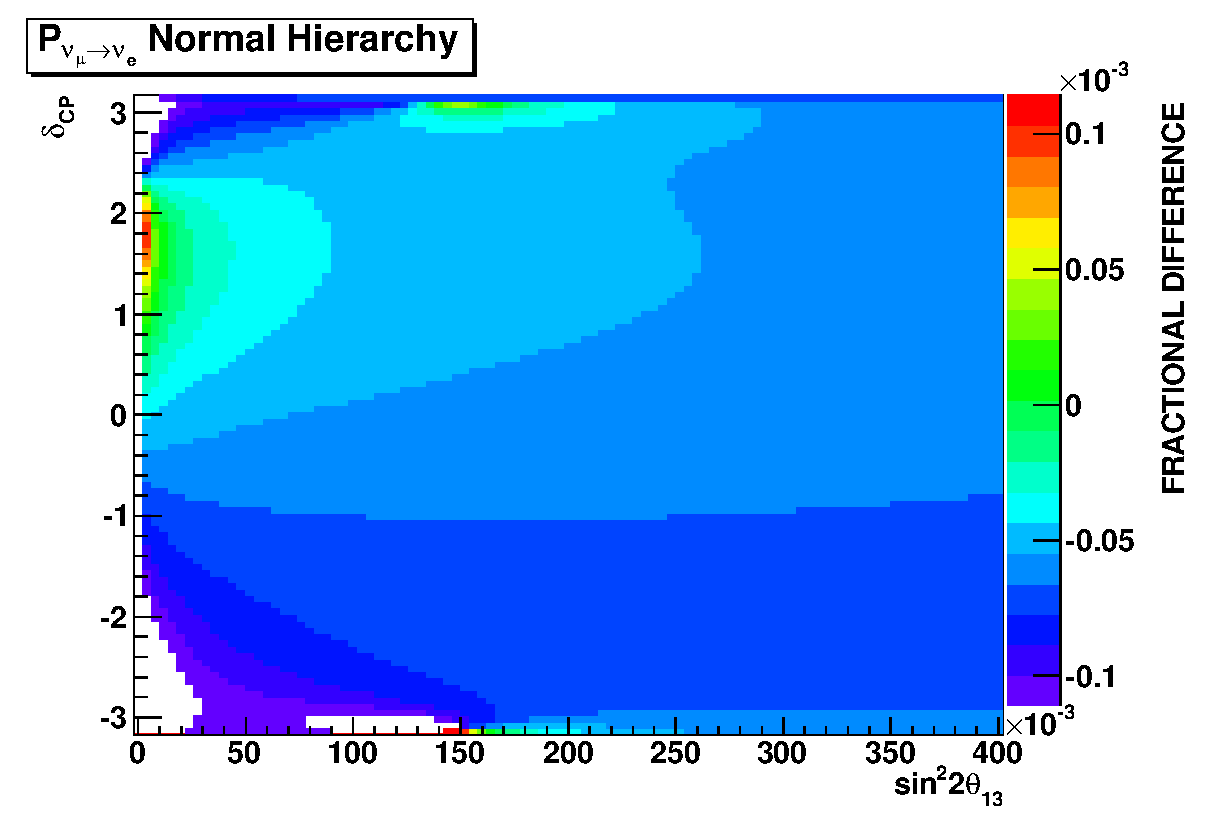
\includegraphics[width=18pc,height=18pc]{./images/osc_prob/prob3_comparison/ComparisonNuMuToNuENH.eps}
\caption{
  Comparison of the VaLOR $\nu_{\mu}\rightarrow\nu_{e}$ oscillation probabilities in matter with those obtained from Prob3++ 
  as a function of $\sin^{2}2\theta_{13}$ and $\delta_{CP}$ for E$_{\nu}$ = 1 GeV; normal mass hierarchy, 
  $\sin^{2}2\theta_{23}$ = 1.0, $|\Delta m_{32}^{2}|$ = 2.4$\times$10$^{-3}$ eV$^{2}$/c$^{4}$, $\sin^{2}2\theta_{12}$ = 0.8704,
  $\Delta m_{21}^{2}$ = 7.6$\times$10$^{-5}$ eV$^{2}$/c$^{4}$ and Earth crust density = 2.6 g/cm$^{3}$.
}
\label{fig:comp_valor_prob3pp_nh_numu_nue}
\end{minipage}
\hspace{0.06\linewidth}
\begin{minipage}[t]{0.47\linewidth}
\centering  
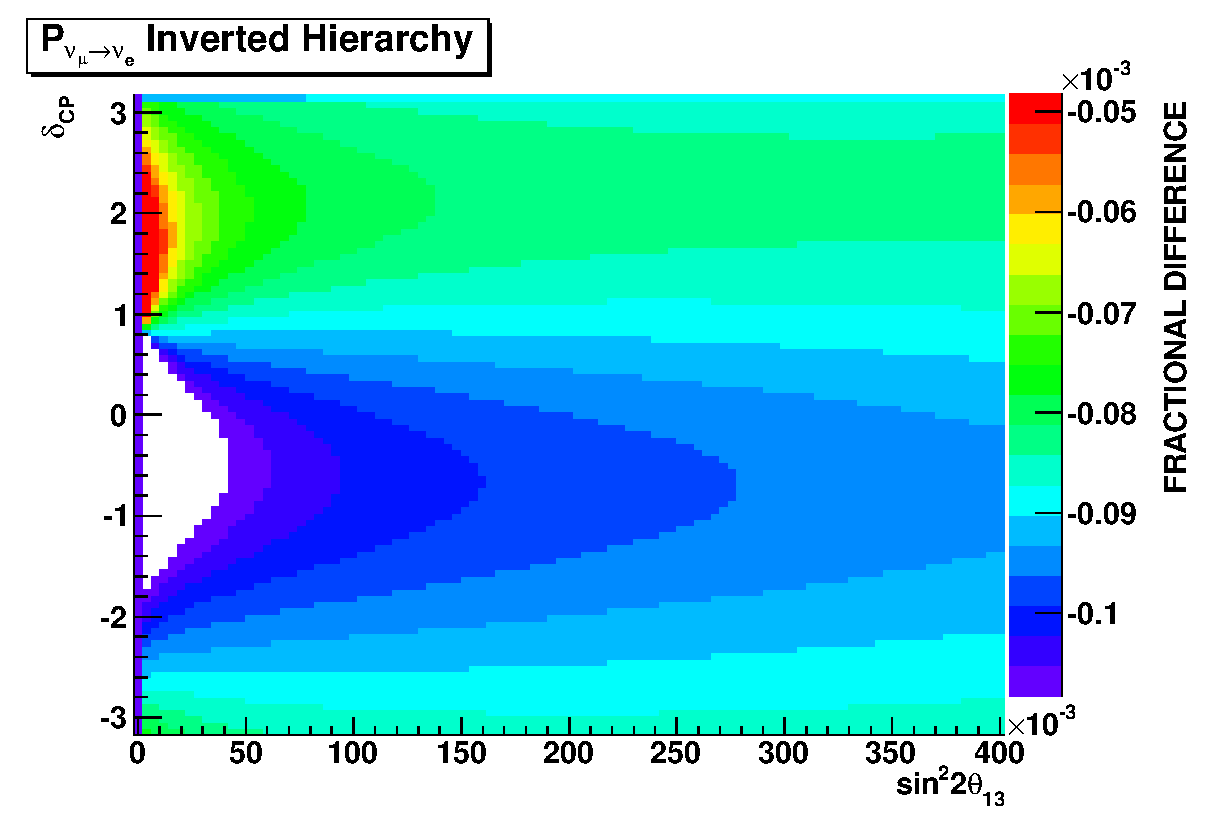
\includegraphics[width=18pc,height=18pc]{./images/osc_prob/prob3_comparison/ComparisonNuMuToNuEIH.eps}
\caption{
  Comparison of the VaLOR $\nu_{\mu}\rightarrow\nu_{e}$ oscillation probabilities in matter with those obtained from Prob3++ 
  as a function of $\sin^{2}2\theta_{13}$ and $\delta_{CP}$ for E$_{\nu}$ = 1 GeV; inverted mass hierarchy, 
  $\sin^{2}2\theta_{23}$ = 1.0, $|\Delta m_{32}^{2}|$ = 2.4$\times$10$^{-3}$ eV$^{2}$/c$^{4}$, $\sin^{2}2\theta_{12}$ = 0.8704, 
  $\Delta m_{21}^{2}$ = 7.6$\times$10$^{-5}$ eV$^{2}$/c$^{4}$ and Earth crust density = 2.6 g/cm$^{3}$.
}
\label{fig:comp_valor_prob3pp_nh_numu_nue}
\end{minipage}
\end{figure}

%
% nue -> numu
%

\begin{figure}[ht]
\begin{minipage}[t]{0.47\linewidth}
\centering
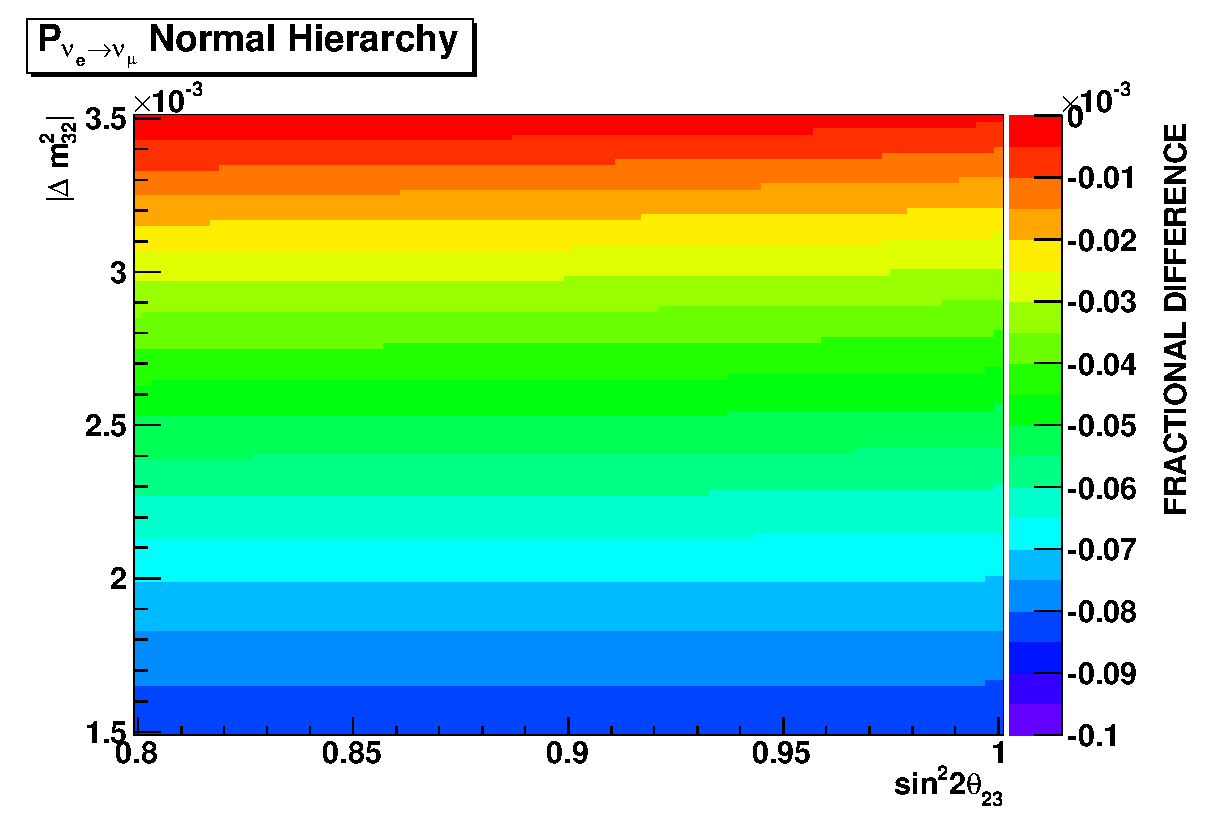
\includegraphics[width=18pc,height=18pc]{./images/osc_prob/prob3_comparison/ComparisonNuEToNuMuNH.eps}
\caption{
  Comparison of the VaLOR $\nu_{e}\rightarrow\nu_{\mu}$ oscillation probabilities in matter with those obtained from Prob3++ 
  as a function of $\sin^{2}2\theta_{23}$ and $|\Delta m_{32}^{2}|$ for E$_{\nu}$ = 1 GeV; normal mass hierarchy, 
  $\sin^{2}2\theta_{13}$ = 0.1, $\sin^{2}2\theta_{12}$ = 0.8704, $\Delta m_{21}^{2}$ = 7.6$\times$10$^{-5}$ eV$^{2}$/c$^{4}$,
  $\delta_{CP}$ = 0 and Earth crust density = 2.6 g/cm$^{3}$.
}
\label{fig:comp_valor_prob3pp_nh_nue_numu}
\end{minipage}
\hspace{0.06\linewidth}
\begin{minipage}[t]{0.47\linewidth}
\centering  
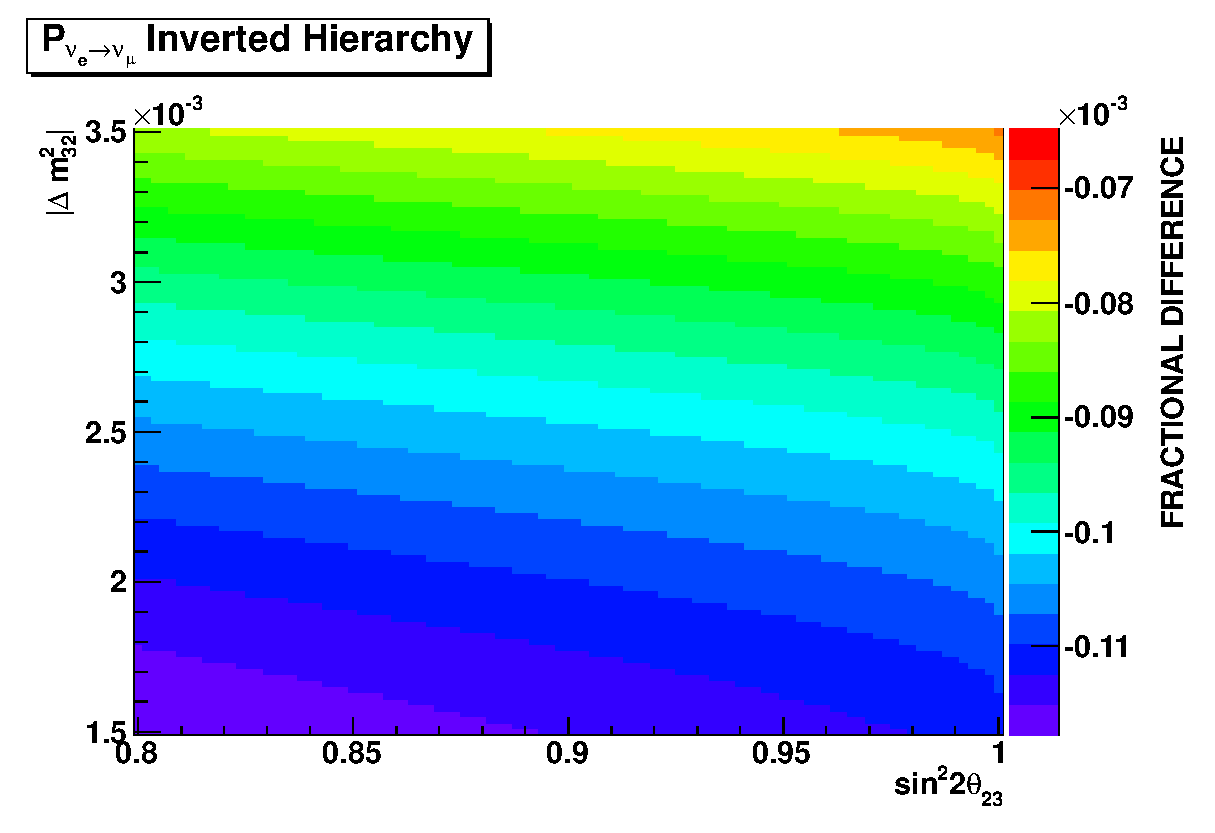
\includegraphics[width=18pc,height=18pc]{./images/osc_prob/prob3_comparison/ComparisonNuEToNuMuIH.eps}
\caption{
  Comparison of the VaLOR $\nu_{e}\rightarrow\nu_{\mu}$ oscillation probabilities in matter with those obtained from Prob3++ 
  as a function of $\sin^{2}2\theta_{23}$ and $|\Delta m_{32}^{2}|$ for E$_{\nu}$ = 1 GeV; inverted mass hierarchy, 
  $\sin^{2}2\theta_{13}$ = 0.1, $\sin^{2}2\theta_{12}$ = 0.8704, $\Delta m_{21}^{2}$ = 7.6$\times$10$^{-5}$ eV$^{2}$/c$^{4}$, 
  $\delta_{CP}$ = 0 and Earth crust density = 2.6 g/cm$^{3}$.
}
\label{fig:comp_valor_prob3pp_nh_nue_numu}
\end{minipage}
\end{figure}


